% created by H. Gu at 9 Nov 22

\documentclass[UTF8]{ctexart}
\usepackage{amsmath}
\usepackage{cite}
\usepackage{graphicx}
\usepackage{array}
\renewcommand\arraystretch{1.1} % 表格行距
\usepackage[a4paper, margin=1in]{geometry}
\usepackage{fancyhdr}
\pagestyle{fancy}
\usepackage{listings}
\usepackage{float}
% \fancyhf{}
%\usepackage[framed,numbered,autolinebreaks,useliterate]{mcode}

\title{\Huge 生物系统建模第二次研讨}
\title{\LARGE 智能手环人体运动状态识别\\
        ~\\
       \Large ——生物系统建模第二次研讨}

\author{\Large XXX 11120101 \\
        \Large YYY 11120121 \\
        \Large ZZZ 11120206  \\
        ~\\
        \Large 生物科学与医学工程学院 \\}
        
\date{\Large \today}


\addcontentsline{toc}{section}{摘要}
\begin{document}
 \fancyhead[L]{ }
\fancyhead[C]{智能手环人体运动状态识别}
\fancyfoot[C]{\thepage}

\maketitle

\newpage
\begin{abstract}
现在市场上有各种各样的智能手环。多数智能手环都具有久坐提醒、运动检测等功能。查阅资料,手环对人体的姿态识别是通过内置加速度计、陀螺仪、GPS等传感器实现的。利用phyphox软件调用手机内置传感器提取数据,并用机器学习算法SVM进行状态分类

关键词:手环,姿态,传感器,SVM
\end{abstract}
\newpage

\tableofcontents
\newpage

\section{背景}

\subsection{手环}
智能手环是可穿戴式智能设备的一种,可以将数据与智能手机等设备同步,具有计步和测量距离、卡路里等基本功能,还具有活动、锻炼、睡眠等模式,可以记录营养情况,拥有智能闹钟、健康提醒、蓝牙4.0数据传输等特殊功能。传感器是可穿戴设备感知外部环境的窗口,也是产品功能差异化的重要硬件,需要有好的算法提高数据精准度。
\subsection{phyphox}
phyphox是一款基于智能手机和平板电脑的科学实验平台,可以将手机、平板电脑等设备转变成数据采集器和实验室工具,用于进行各种物理实验和数据收集。它提供了大量的传感器和功能,可以测量、记录或计算各种物理量,如加速度、角速度、磁场、光强、声音等,同时得到的数据可以导出到CSV,Excel或文本文件中,方便后续的数据分析和处理。
\cite{Georgopoulos1982}

\subsection{SVM算法}
SVM(支持向量机,Support Vector Machine)是一种常见的机器学习算法,其主要用于二分类问题和回归问题。SVM 通过将数据映射到高维空间来寻找一个最优的超平面,以将不同类别的样本分开。以下是一些关于 SVM 的介绍:\\
1. SVM 的核心思想是寻找一个最优的超平面来将不同类别的样本区分开。对于线性可分的情况,SVM 可以找到一个线性超平面来实现分类;对于非线性可分的情况,SVM 可以通过核函数将原始数据映射到高维特征空间中,从而找到一个非线性超平面。\\
2. SVM 的只关注距离超平面最近的一些点,这些点被称为支持向量。在训练模型时,SVM 会通过最大化支持向量到超平面的距离(即间隔)来寻找最优的超平面。\\
3. SVM 还具有一个重要的参数 C,它控制了模型的复杂度。当 C 很小时,SVM 会选择较简单的模型,减少过拟合的风险;而当 C 很大时,SVM 会选择更复杂的模型,提高模型的泛化能力。\\
4. SVM 还可以通过使用核函数来处理非线性问题。常用的核函数包括线性核、多项式核、高斯核等,它们可以将原始数据映射到高维空间中,以便 SVM 寻找一个非线性的超平面。SVM 是一种非常流行的机器学习算法,其通过寻找最优的超平面来实现数据分类和回归。SVM 不仅适用于线性可分问题,还可以通过核函数处理非线性问题,具有很强的泛化能力。
\begin{figure}[H]
    \centering
    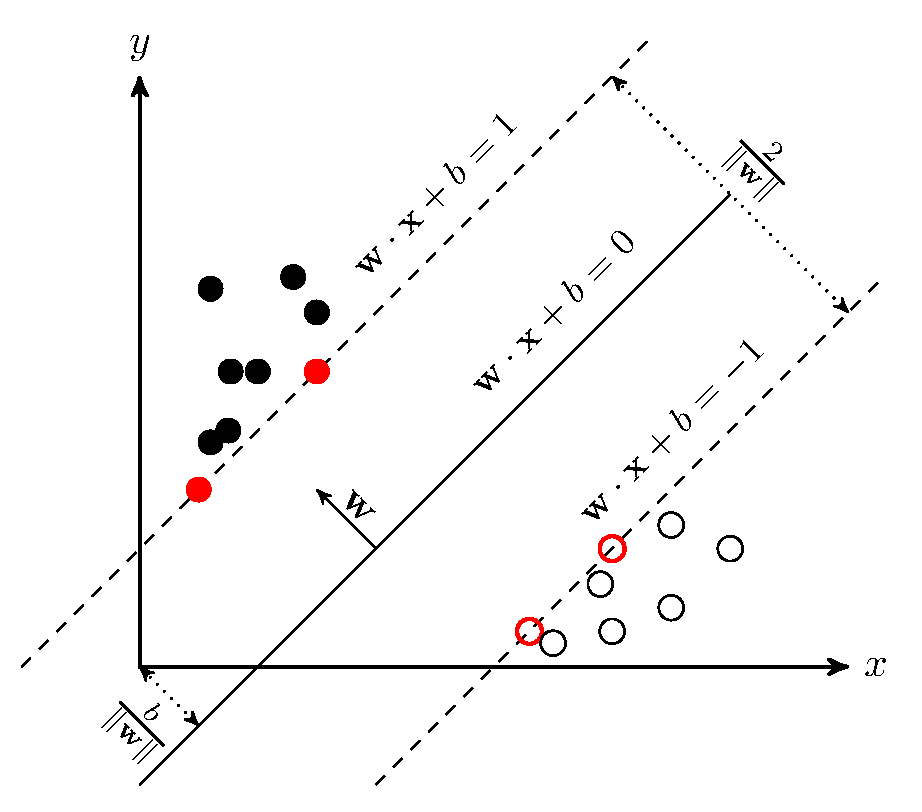
\includegraphics[width=0.6\textwidth]{pic/SVM原理示意图.png}
    \caption{SVM原理示意图}
    \label{fig:demo}
\end{figure}

\section{环境配置及说明}
\subsection{环境配置}

\begin{table}[H]
    \centering
    \caption{环境配置}
    \begin{tabular}{ccccc}
    \hline
    No  & $Environment$    & $Version$     \\
    \hline
    1   & Windows  & 11  \\ 
    2   & Python  & 3.11 \\ 
    % 3   & Anaconda3 & 2023.03  \\ 
    % 4   & Pycharm  & Community2023.1\\
    % 5   & Cuda  & 12.1  \\ 
    % 6   & Pillow & 9.5.0  \\ 
    3   & Pip  & 23.1  \\ 
    4   & scikit-learn  & 1.2.2  \\ 
    5   & pandas & 2.0.1 \\
    % 9   & TensorFlow  & 2.12.0  \\ 
    % 10   & numpy  & 3.2.2  \\ 
    \hline
    \end{tabular}   
  \label{tab1}
\end{table}

\subsection{函数库说明}
Scikit-learn是一款Python机器学习库,它提供了大量的算法和工具,用于分类、聚类、回归和降维等任务。Scikit-learn的主要优点包括以下几点:

1.	易于学习和使用:Scikit-learn提供了Python的API接口,易于Python程序员学习和使用,同时还有丰富的文档和代码示例,使得入门门槛较低。

2. 统一的API设计:Scikit-learn采用了统一的API设计,使得不同算法之间切换变得容易,还可以通过封装来简化模型训练的流程。

3.	丰富而又完整的算法实现:Scikit-learn提供了多种经典和先进的机器学习算法的实现,如逻辑回归、决策树、支持向量机、随机森林、神经网络等,而且这些算法的实现都是经过优化和高度可靠性的。

因此,Scikit-learn成为了一个备受欢迎的开源机器学习库,被广泛应用于数据处理、特征提取、预测建模等领域。

Scikit-learn也被广泛应用于图像处理方面的任务,这是因为Scikit-learn提供了许多常用的图像处理函数和算法,如PCA、LDA、KNN等,能够帮助开发人员进行图像分类、聚类和降维等任务。同时,Scikit-learn还提供了丰富的特征提取和数据预处理方法,使得机器学习模型在图像处理的任务中表现得更加优秀。

\section{数据采集和数据预处理}
\subsection{数据采集}
本实验用phyphox调用手机内置GPS、陀螺仪,加速度传感器采集数据,站立,正坐,走动,跑动各20min,导出数据,各传感器包含数据如下:

\begin{table}[H]
    \centering
    \caption{各传感器数据}
    \begin{tabular}{ccccc}
    \hline
    Name\\  %& $U$    & $I$    & $R$   & $\Delta R$ \\
    \hline
    Accelerometer   & Time(s) & X($rad/s^2$)  & Y($rad/s^2$)  & Z$(rad/s^2$) \\ 
    Liner Accelerometer   & Time(s) & X($rad/s^2$)  & Y($rad/s^2$)  & Z$(rad/s^2$) \\  
    Gyroscope  & Time(s) & X(rad/s)  & Y(rad/s)  & Y(rad/s) \\  
    Location & Time(s) & Latitude(°)  & Longitude(°) & Height(m)\\
    \hline
    \end{tabular}
\end{table}

\subsection{数据预处理}
去掉数据中的第一行和第一列,按照每个文件包含 100 行(处理location时为10行,下同)的方式进行拆分,拆分后的文件保存到指定的文件夹中。最后,因为最后一个组的数据可能小于100行,所以需要进行特殊处理,选中组后一组的所有行并生成新数据。训练集和测试集按照9:1划分。


\section{模型辨识}
\subsection{训练集数据加载}
用 Pandas 库读取指定目录下的 csv 文件,并将其整合成一个大的 DataFrame。首先创建一个空的 DataFrame,用于存放读取的所有数据。循环读取根目录下的四个子目录,label 代表标签值(即类别编号),label\_ name 代表标签名。拼接标签目录的完整路径,循环遍历标签目录下的所有文件名,如果文件名以 .csv 结尾,说明是数据文件,进入下一步处理。拼接数据文件的完整路径。读取数据文件,将数据文件的标签值添加到 DataFrame 的最后一列。当前文件读取的 DataFrame 添加到总的 DataFrame 中,按行拼接。最终,DataFrame 中的每一行都代表一个数据样本,其中包含了加速度计和陀螺仪的数据以及其所属的类别。代码如下:\\
\begin{lstlisting}[language=python, basicstyle=\ttfamily]
 root_dir = r'E:\Phyphox\AC'
 all_data = pd.DataFrame()
 for label, label_name in enumerate(['running', 'sitting', 'standing', 'walking']):
 label_dir_path = os.path.join(root_dir, label_name)
    for file_name in os.listdir(label_dir_path):
     if file_name.endswith('.csv'):
        file_path = os.path.join(label_dir_path, file_name)
        data = pd.read_csv(file_path, header=None)
        data['label'] = label
        all_data = pd.concat([all_data, data], axis=0)
\end{lstlisting}

\subsection{准备训练集数据}
首先,从之前加载的所有数据中分离出特征和标签,其中特征是除了最后一列以外的所有列,标签是最后一列。然后,使用train\_ test\_ split函数将数据划分为训练集和验证集,其中test\_ size=0.1表示将10\% 的数据划分到验证集中,random\_ state=42表示设置随机种子,以确保每次运行时数据集的划分是相同的。最终,得到训练集的特征数据X\_ train、训练集的标签数据y\_ train、验证集的特征数据X\_ val和验证集的标签数据y\_ val。代码如下:
\begin{lstlisting}[language=python, basicstyle=\ttfamily]
 X = all_data.iloc[:, :-1]
 y = all_data.iloc[:, -1]
 X_train, X_val, y_train, y_val = train_test_split(X, y, test_size=0.1,     
  random_state=42)
\end{lstlisting}
\subsection{训练模型}
首先,创建一个SVC对象svm\_ model作为模型,使用径向基核函数,表示正则化参数设置为1,核函数的系数设置为0.1。然后,使用fit函数将训练集的特征数据X\_train和标签数据y\_ train输入到模型中进行训练,从而得到训练好的模型。代码如下:\\
\begin{lstlisting}[language=python, basicstyle=\ttfamily]
 svm_model = SVC(kernel='rbf', C=1, gamma=0.1)
 svm_model.fit(X_train, y_train)
\end{lstlisting}

\subsection{测试模型}
定义一个变量test\_ dir表示测试集数据所在的文件夹路径。然后,创建一个空列表pred\_ labels用于保存预测结果。接着,遍历测试集文件夹中的所有.csv文件,读取文件数据并使用已经训练好的模型进行预测,将预测结果添加到pred\_ labels列表中。最终,在pred\_ labels列表中保存所有测试数据对应的预测结果。代码如下\\
\begin{lstlisting}[language=python, basicstyle=\ttfamily]
  test_dir = r'E:\Phyphox\filepro\test\Accelerometer'
  pred_labels = []
  for file_name in os.listdir(test_dir):
    if file_name.endswith('.csv'):
        file_path = os.path.join(test_dir, file_name)
        test_data = pd.read_csv(file_path, header=None)
        pred_label = svm_model.predict(test_data)
        pred_labels.append(pred_label[0])
\end{lstlisting}

\subsection{预测输出结果}
首先定义一个包含四个标签名的列表 label\_ names,然后在一个循环中遍历测试数据文件夹中的所有 CSV 文件,读取数据并使用训练好的 SVM 模型进行预测,将预测结果(一个整数)添加到一个列表 pred\_ labels 中。接着,将预测结果转换为标签名,并将它们写入到一个的文本文件中,每个标签名占一行。代码如下:\\
\begin{lstlisting}[language=python, basicstyle=\ttfamily]
  label_names = ['running', 'sitting', 'standing', 'walking']
  pred_label_names = [label_names[i] for i in pred_labels]
  with open('predictions2.txt', 'w') as f:
    for pred_label_name in pred_label_names:
        f.write(pred_label_name + '\n')
\end{lstlisting}

\section{模型验证}
采集坐姿,站姿,走路,跑步数据各1min进行测试。
\subsection{通过Acceleration预测}
\begin{figure}[H]
    \centering
    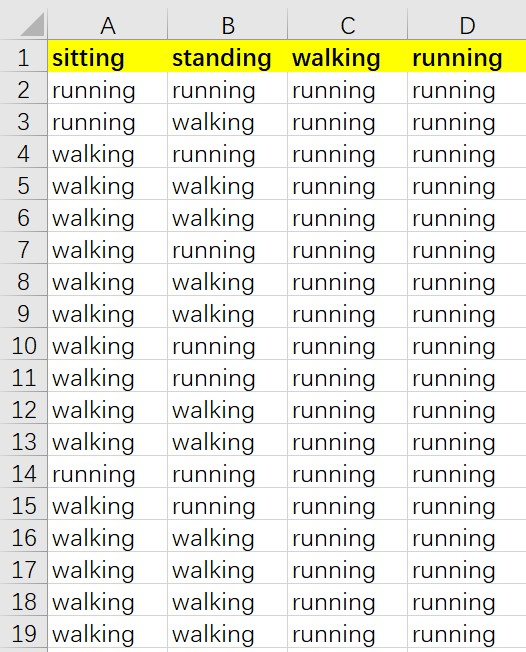
\includegraphics[width=0.5\textwidth]{pic/pre_a.jpg}
    \caption{SVM原理示意图}
    \label{fig:demo}
\end{figure}

\subsection{通过Liner-Acceleration预测}
\begin{figure}[H]
    \centering
    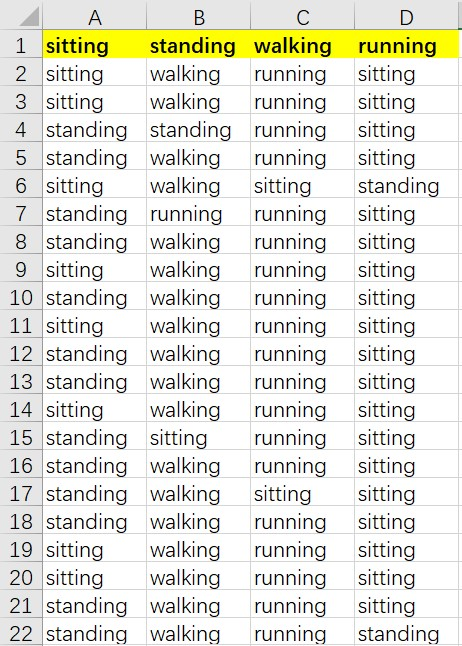
\includegraphics[width=0.5\textwidth]{pic/pre_LA.jpg}
    \caption{SVM原理示意图}
    \label{fig:demo}
\end{figure}

\subsection{通过Location预测}
\begin{figure}[H]
    \centering
    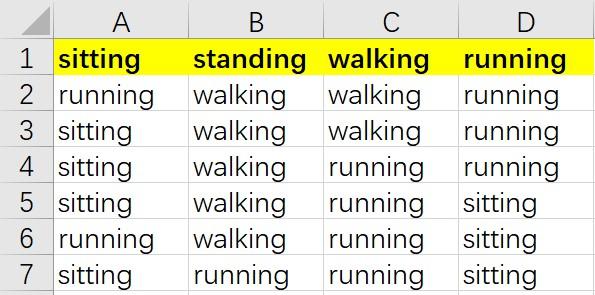
\includegraphics[width=0.5\textwidth]{pic/pre_loc.jpg}
    \caption{SVM原理示意图}
    \label{fig:demo}
\end{figure}

\subsection{通过Gyroscope预测}
\begin{figure}[H]
    \centering
    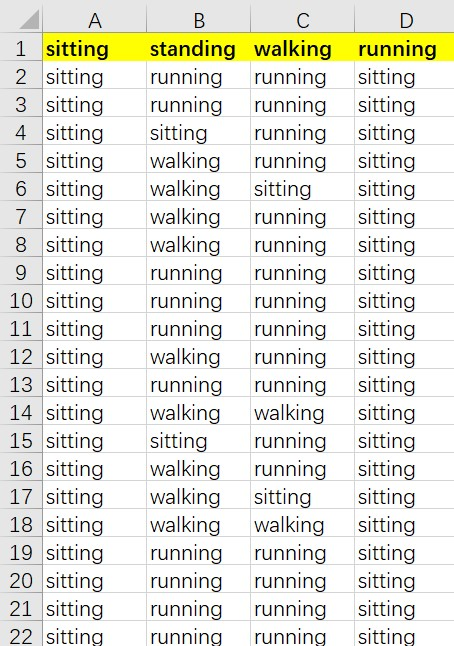
\includegraphics[width=0.6\textwidth]{pic/pre_Gyr.jpg}
    \caption{SVM原理示意图}
    \label{fig:demo}
\end{figure}
\section{分析与讨论}
1. 采集到的数据并未进行滤波处理,噪声较大,影响了准确率。

2. 数据特征不明显。使用加速度进行分类时,由于坐姿,站姿的加速度都为0,二者仅依靠加速度无法区分,所以无法进行四分类,而跑步和走路二者加速度区别较大。应当增加特征值,综合各个传感器的数据进行分类学习。

3. 使用陀螺仪进行分类时,四种姿势的手臂状态会有明显差异,可以根据朝向和角速度区分四类状态,但是跑步运动伴有手臂倾角,一定程度上影响了准确性。

4. 对于此类非线性的数据,可以采用决策树、随机森林、神经网络等其他分类器提高准确率。




\end{document}
